\pagebreak{}

Consider the blood cell iterative equation $c_{n+1} = (1-a)c_{n}+bc_{n}^{r}e^{-sc_{n}}$.

\section*{Iterative Numerics}
\textbf{Question 1:} Run iterative numerics and describe different types of trajectories.

\textbf{Answer:} 
\begin{figure}[H]
	\begin{center}
    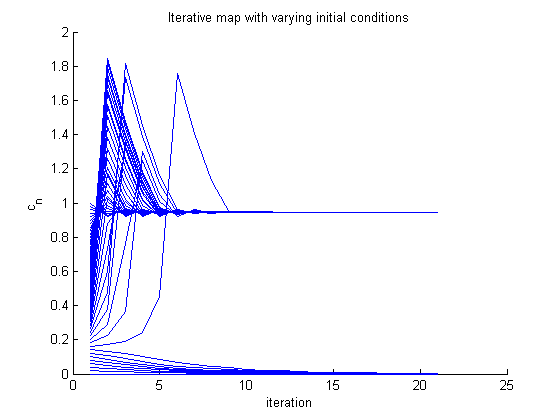
\includegraphics[width=0.8\textwidth]{IterativeNumerics}
    \end{center}
    \caption{Map with 20 different initial conditions, with a = 0.2.}
    \label{Fig. 1}
\end{figure}
Figure 1 plots the map for 20 different initial conditions using typical parameters as described by Lasota in 1977, namely: $b=1.1*10^{-6}, \quad r=8, \quad s=16$. Other possible parameter regimes have also been discussed by Steven Lynch. In general, $a \in [0,1]$, but the `$a$' parameter was chosen in this case to be in a region where the system can converge to one of two stable fixed points depending on the initial conditions. 

\begin{figure}[H]
	\center{center}
    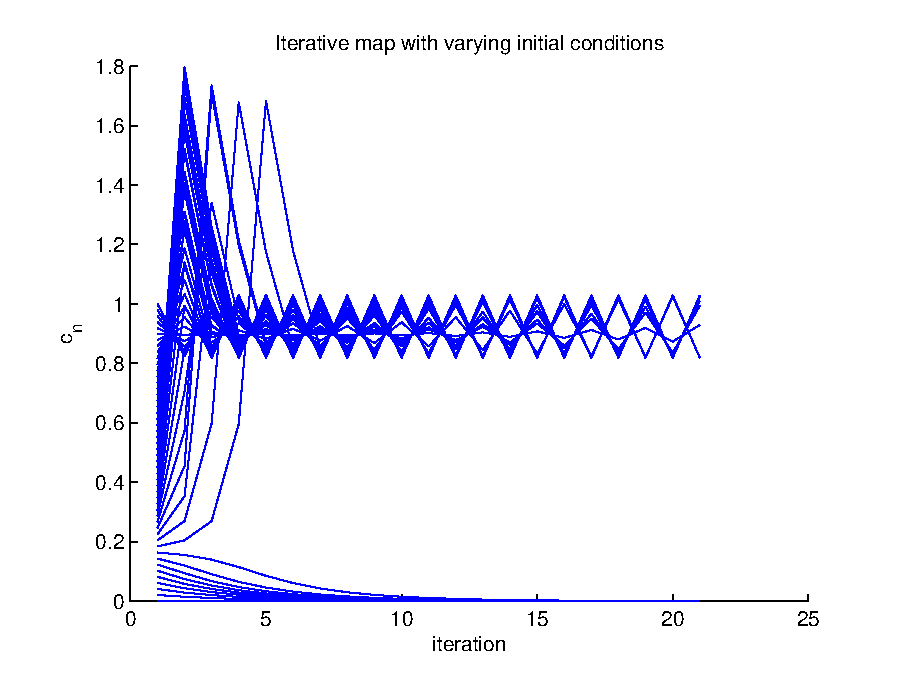
\includegraphics[width=0.8\textwidth]{IterativeNumericsa03}
    \center{center}
    \caption{Map with 20 different initial conditions with parameter a being changed to 0.3.}
    \label{Fig. 2}
\end{figure}
The only change made from figure 1 to figure 2 was the parameter `$a$'. It now lies in a region with one stable solution and a 2-periodic solution. Figure 3 captures all of the behaviours that the system exhibits upon varying '$a$' and the initial condition. At the bottom of the bifurcation diagram we can see that a single stable solution that goes to 0. As '$a$' increases we see orbits of periods 2, 4, and 8 emerge. Then, undoubling of orbits occurs until $a\approx.7$ at which point we see bistability takes place. Figure 4 zooms in on the bistable region. Period doubling begins again at $a\approx .715$ before the system then goes to chaos, but sporadic instances of high periodicity orbits occur for $a \in (.725, .84)$. Figure 5 shows the system eventually becoming a single stable solution at $c_n=0$ for large enough '$a$' and any initial condition. 

\begin{figure}[H]
    \begin{center}
    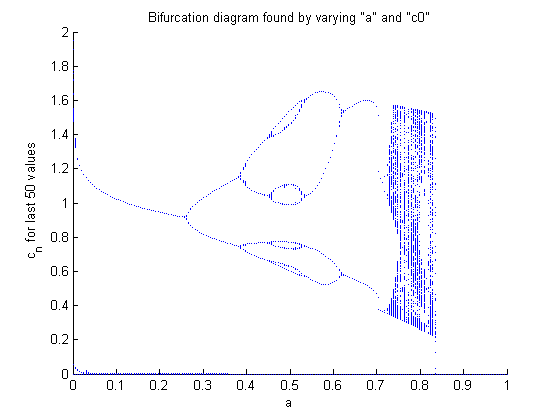
\includegraphics[width=0.8\textwidth]{Varyac0}
    \end{center}
    \caption{Behaviors of the system exhibited by varying initial conditions.}
    \label{Fig. 3}
\end{figure}
\begin{figure}[H]
	\begin{center}
    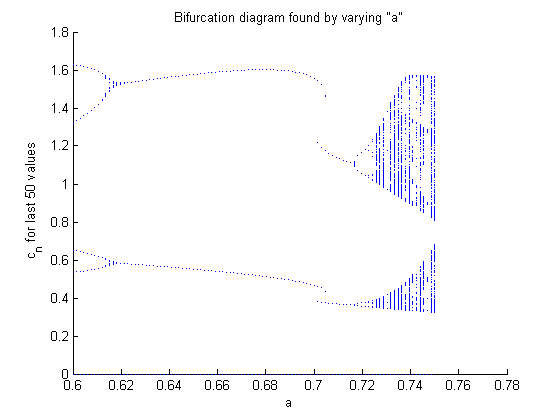
\includegraphics[width=0.8\textwidth]{BistableRegion}
    \end{center}
    \caption{Bistable Region}
    \label{Fig. 4}
\end{figure}
\begin{figure}[H]
    \begin{center}
    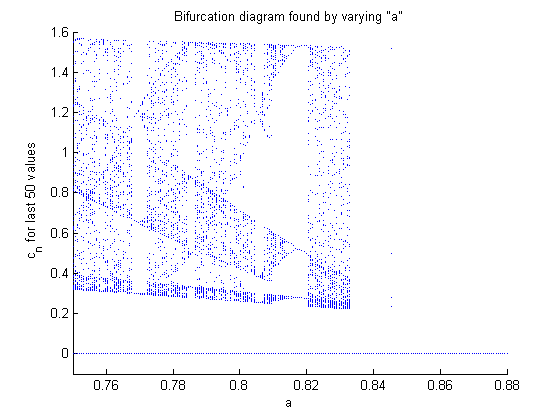
\includegraphics[width=0.8\textwidth]{chaostoStable}
    \end{center}
    \caption{Chaotic to Stable Behavior}
    \label{Fig. 5}
\end{figure}
